\section{Displej}
Aby byl budík uživatelsky přívětivý, je nutné umožnit jeho nastavování bez
nutnosti připojení jiného zařízení (počítače, mobilního telefonu apod.).
Pro zobrazování dat se v dnešní době využívá široká škála různých technologií
displejů. Vzhledem k textovému charakteru zobrazovaných dat jsou pro toto
zařízení vhodné znakové či grafické displeje, segmentové displeje by neumožnily
zobrazení většího množství údajů na jednom místě. Protože není potřeba
zobrazovat složitou grafiku, zvolil jsem znakový LCD displej (16 znaků na
řádek, 2 řádky) s řadičem HD44780. Ten je asi nejlevnější alternativou, je
snadno dostupný a díky možnosti nadefinovat několik vlastních znaků lze
zobrazovat i jednoduchou grafiku.

Řadič HD44780 využívá pro komunikaci 8bitovou sběrnici ($\mathrm{DB0}$ až
$\mathrm{DB7}$) a tři řídicí piny: $\mathrm{R}/\overline{\mathrm{W}}$,
$\mathrm{E}$ a $\mathrm{RS}$. Pin $\mathrm{R}/\overline{\mathrm{W}}$ určuje,
jestli požaduje mikrokontrolér čtení dat z řadiče (logická 1) či zápis (logická
0). V obou případech se data přenášejí po sběrnici. Pin $\mathrm{E}$ zahajuje
operaci čtení či zápisu. $\mathrm{RS}$ určuje, jestli jsou data na sběrnici
daty pro zápis do paměti řadiče ($\mathrm{RS} = 1$, obvykle zápis ASCII hodnoty
požadovaného znaku) nebo instrukce, kterou má řadič provést ($\mathrm{RS} =
0$). Podporované instrukce zahrnují smazání displeje, zapnutí blikání kurzoru
apod. Řadič umožňuje i provoz ve 4bitovém režimu, v takovém případě se ze
sběrnice využijí pouze piny $\mathrm{DB4}$ až $\mathrm{DB7}$.~\cite{dshHD44780}

Pro nedostatek I/O portů použitého MCU je displej připojen přes
8bitový \IIC{} I/O expandér PCF8574. Komunikace s řadičem
HD44780 probíhá vzhledem k malému počtu dostupných pinů ve 4bitovém režimu.
Expandér PCF8574 má 8 pinů, které lze nezávisle nastavit jako vstup či výstup.
Výstupní pin $\overline{\mathrm{INT}}$ může být využit pro spuštění
hardwarového přerušení (interrupt) na straně MCU při změně stavu vstupních
pinů, MCU tedy nemusí pravidelně kontrolovat jejich stav.~\cite{dshPCF8574}
Tato funkce ale není při ovládání LCD využita.

\begin{figure}[htbp]
    \centering
    \tikzstyle{box}=[draw, rounded corners=2mm, font={\bfseries}, align=center, inner sep=3mm]
    \begin{tikzpicture}[>=latex]
        \node [box] (mcu) at (0,0) {MCU};
        \node [box] (PCF8574) at (3.5,0) {PCF8574};
        \node [box] (HD44780) at (8,0) {HD44780};
        \node [box] (lcd panel) at (12,0) {LCD panel};
        \draw [->] (mcu) -- (PCF8574)
            node [midway, below] {\footnotesize \IIC{}}
            ;
        \draw [->] (PCF8574) -- (HD44780)
            node [midway, below, align=center, font={\footnotesize}] {4bitová\\paralelní\\sběrnice}
            ;
        \draw [->] (HD44780) -- (lcd panel)
            node [midway, below, align=center, font={\footnotesize}] (lcd rizeni) {řízení\\jednotlivých\\segmentů\\LCD}
            ;
        \node [draw, dashed, inner sep=2mm, fit={(lcd panel) (HD44780) (lcd rizeni)}] (lcd) {}
            node[above, font={\bfseries}] at (lcd.north) {LCD modul};
        \node [draw, dashed, inner sep=2mm, fit={(PCF8574)}] (io expander) {}
            node[above, font={\bfseries}] at (io expander.north) {Modul I/O expandéru};
    \end{tikzpicture}
    \caption{Blokové schéma znázorňující způsob připojení LCD k MCU}
    \label{fig:LCD blok}
\end{figure}


Expandér ovládá také podsvícení displeje. To je zajištěno elektroluminiscenční
diodou (LED) svítící z boku do plexiskla pod open cell (viz rozebrané LCD na
obrázku~\vref{fig:LCD modifikace}). V běžně prodávaných znakových LCD jsou
osazovány bílé LED, přičemž vlastní open cell je modrý. Pro použití
v prostředí s nízkou intenzitou osvětlení se ale považuje za vhodnější
podsvícení červenou barvou.\todo{ozdrojovat modre svetlo v noci} Když pro
podsvícení použijeme červenou LED, blokuje open cell většinu světla a ven
z panelu vychází červené světlo pouze v místech, kde jsou otevřené pixely.

\subsection{Změna barvy podsvícení displeje}
Modifikace barvy podsvícení není triviální, protože se na trhu vyskytuje mnoho
displejů se stejnými rozměry, komunikačním rozhraním apod., ale s rozdílným
provedením podsvětlení (BLU). U všech autorem zakoupených displejů je
podsvícení řešenou jednou LED zapuštěnou do plexiskla na pravé straně displeje.
LED je na desce plošných spojů připájena do prokovených děr, které jsou na
hraně DPS přesně ve své polovině odfrézovány. Důvod pro toto řešení je
pravděpodobně zjednodušení montáže při výrobě. Jednotlivé displeje se liší
tvarem plexiskla a montáží LED do tohoto plexiskla.

\begin{figure}[htbp]
    \centering
    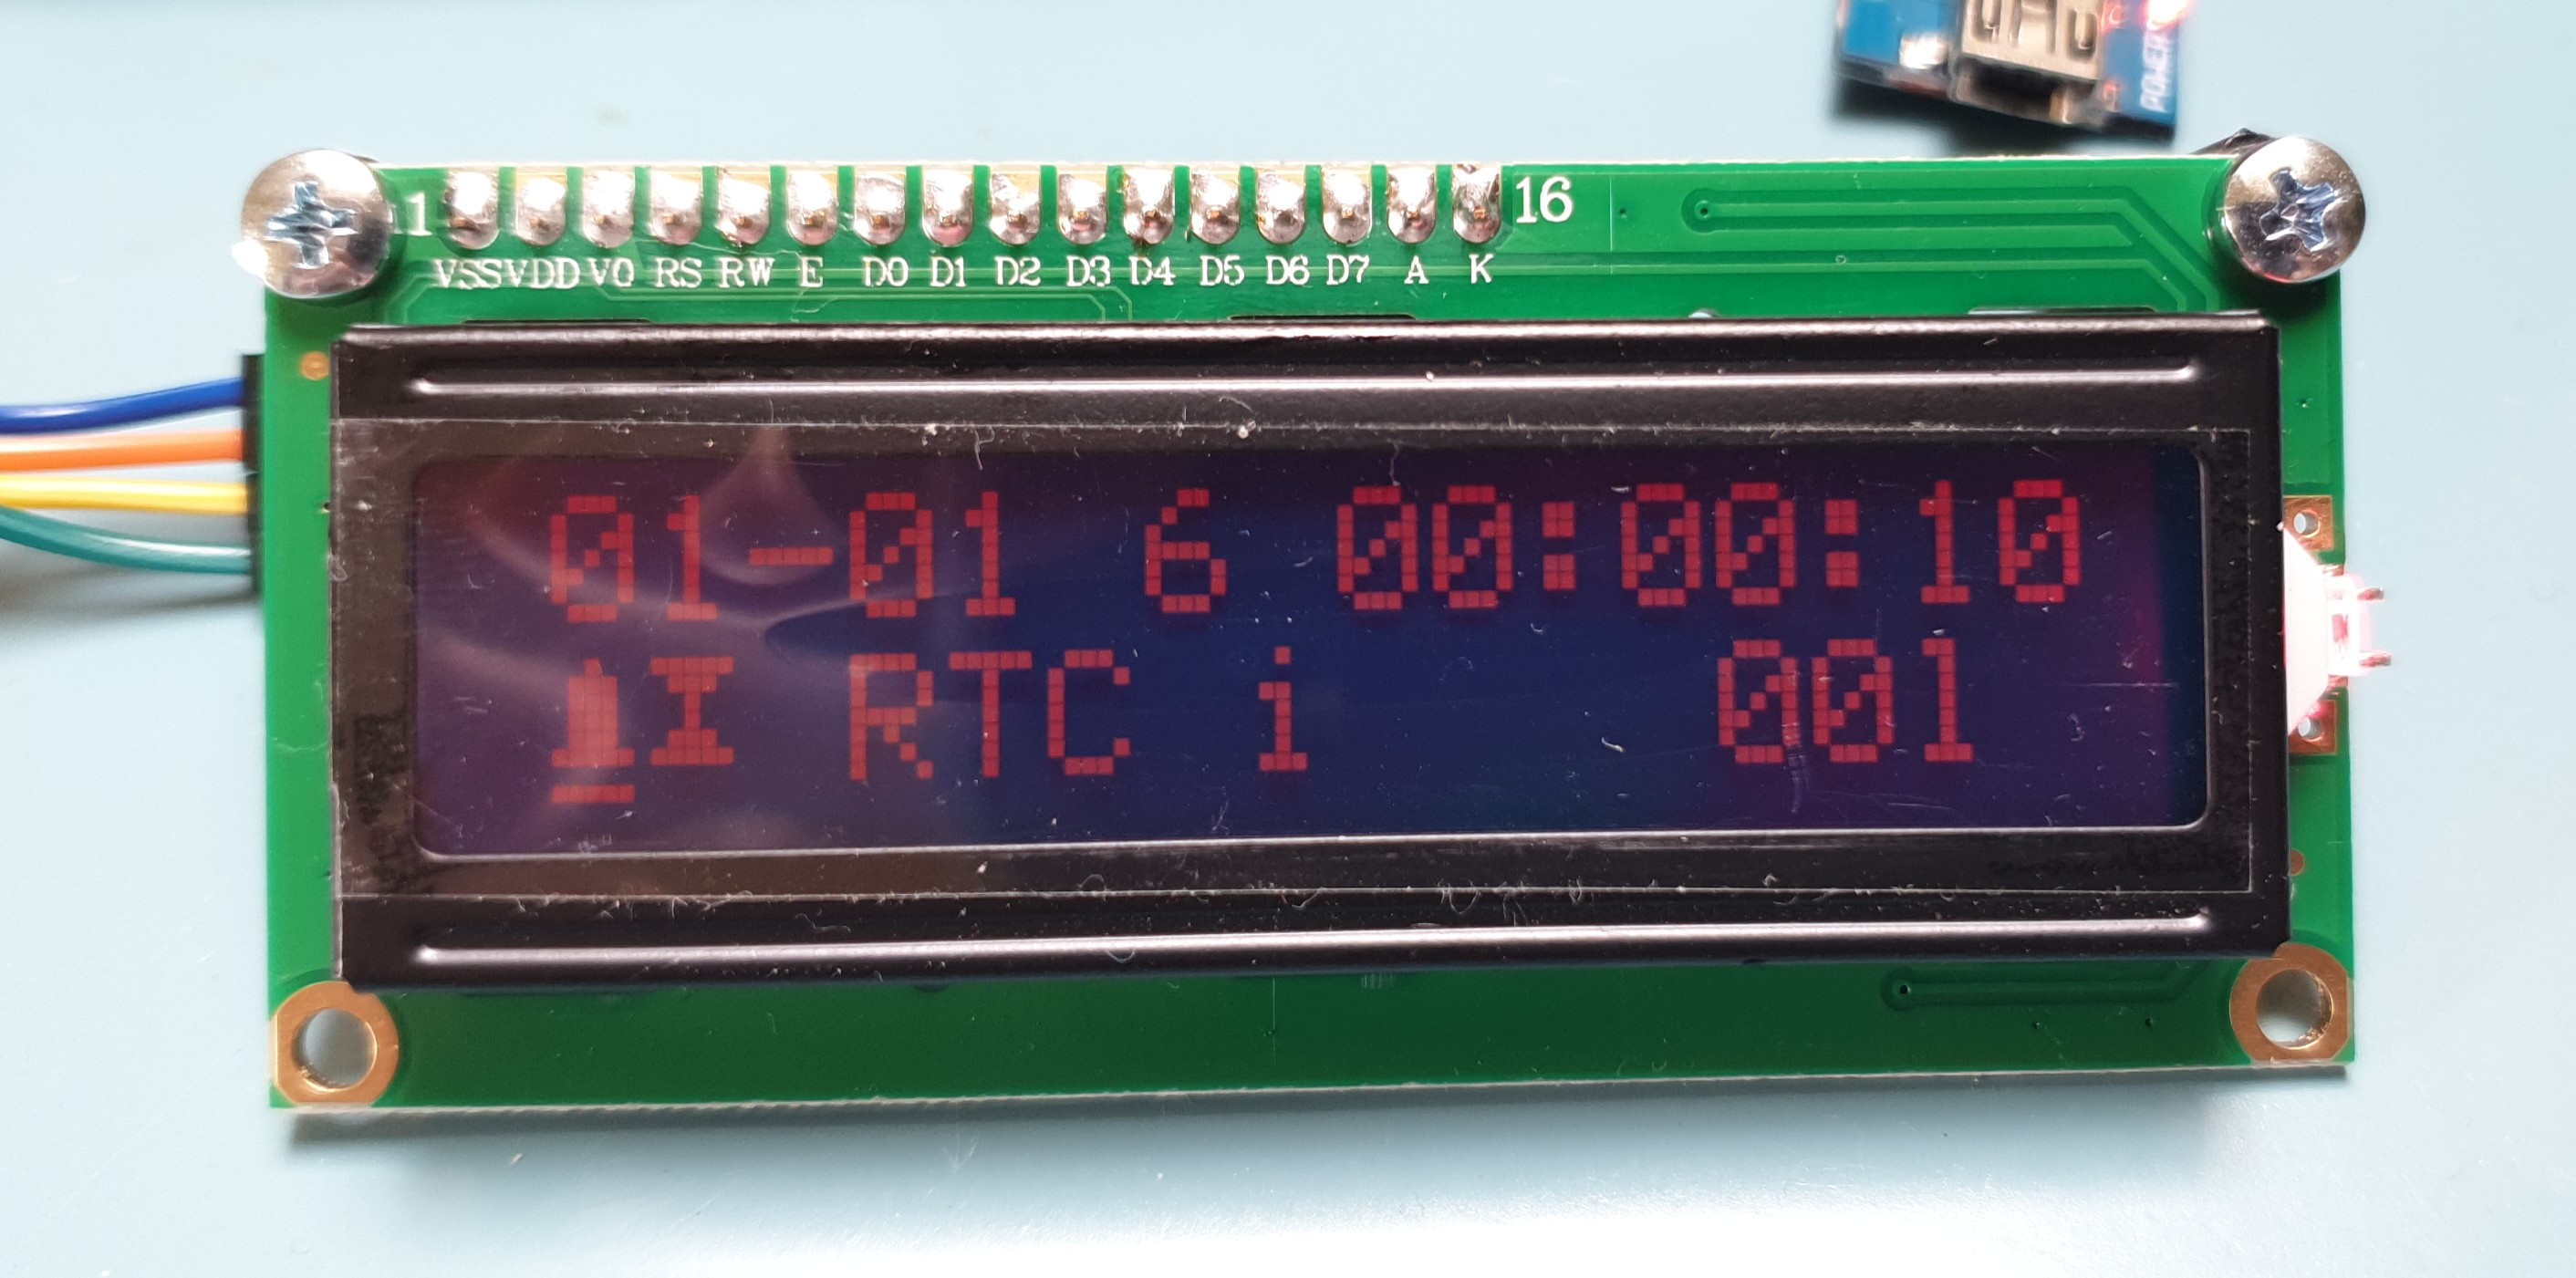
\includegraphics[width=0.7\textwidth]{figures/LCD-mod-after}
    \caption{LCD po změně barvy podsvícení}
    \label{fig:LCD cervena}
\end{figure}

\begin{figure}[htbp]
    \centering
    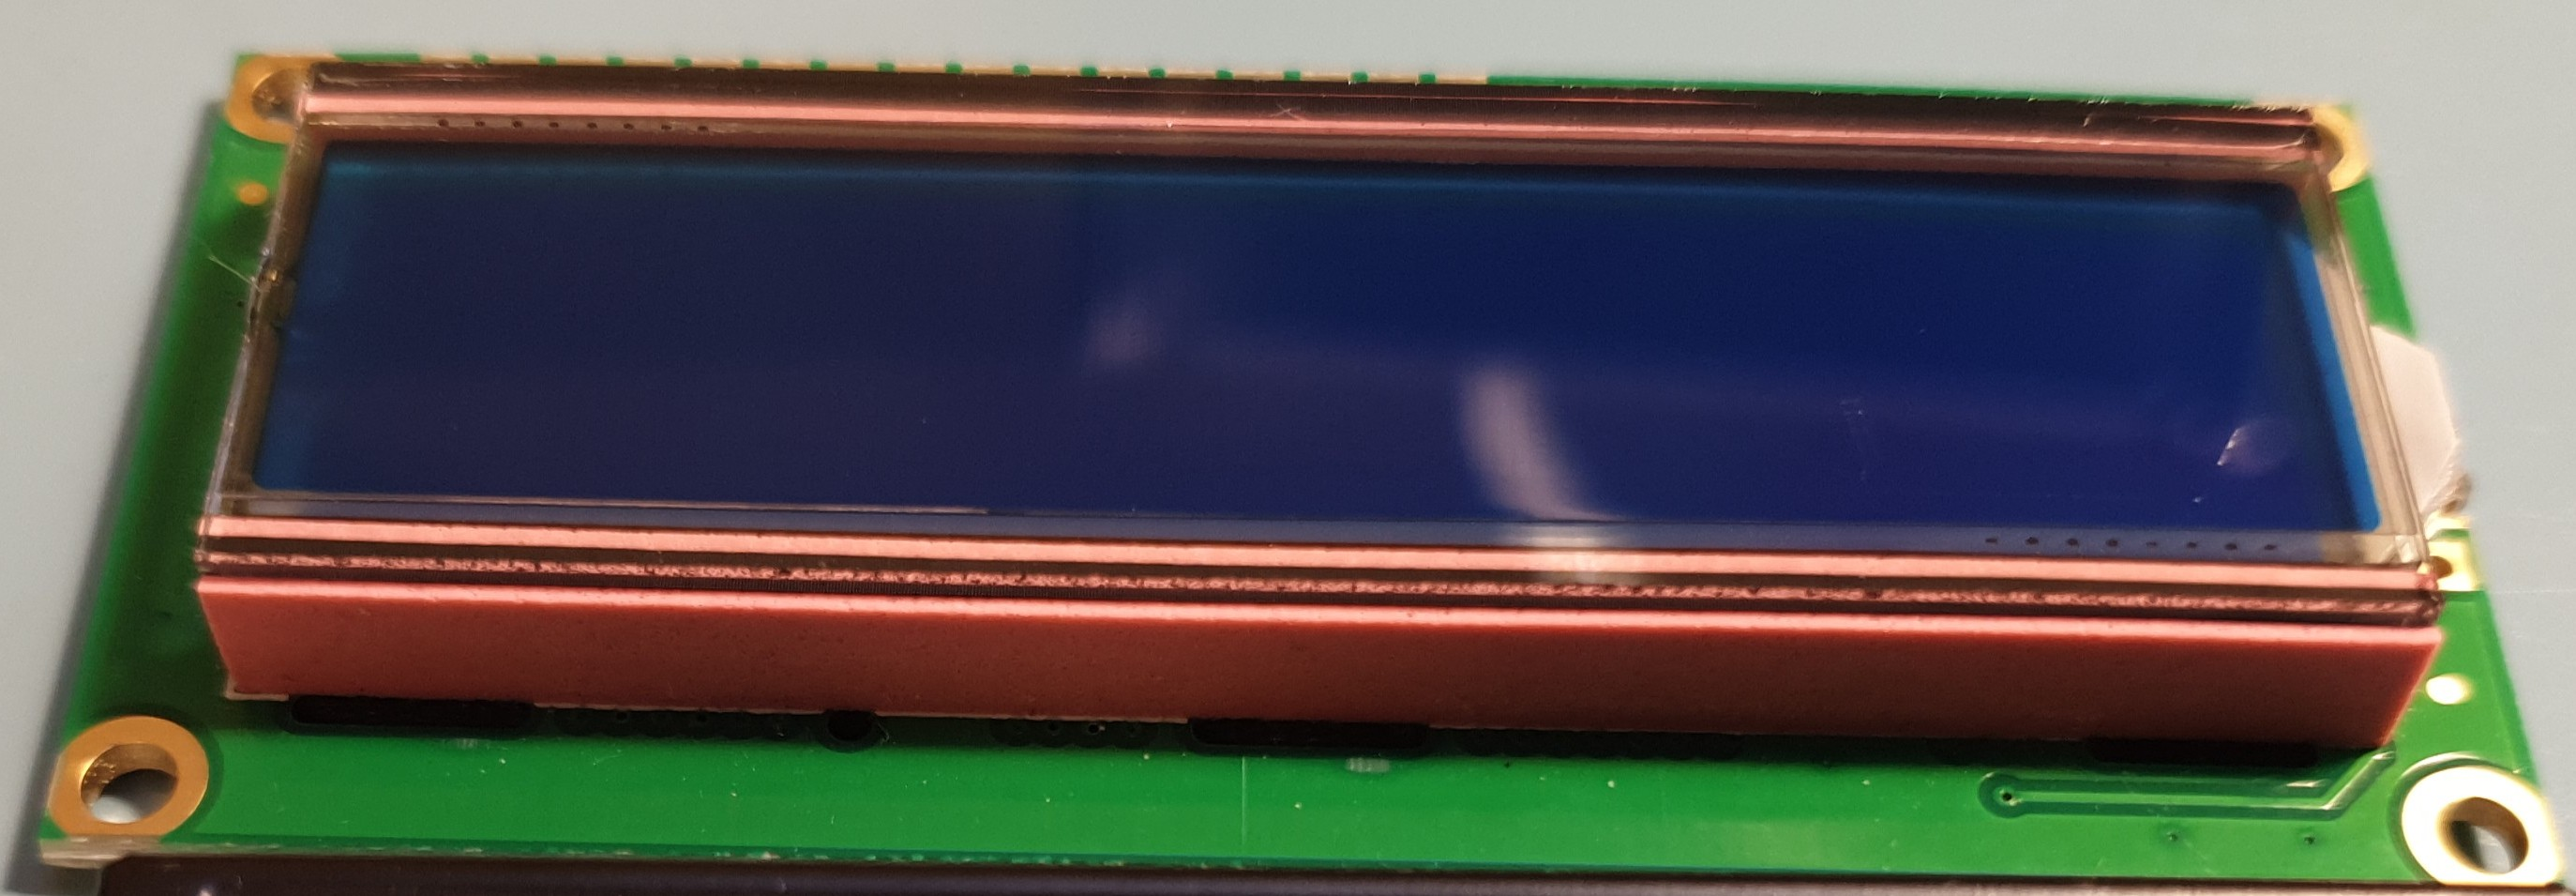
\includegraphics[width=0.8\textwidth]{figures/LCD-mod-disassembly}
    \includegraphics[width=0.8\textwidth]{figures/LCD-mod-BLU-sheet}
    \begin{tikzpicture}
        \node [above right, inner sep=0] (image) at (0,0) {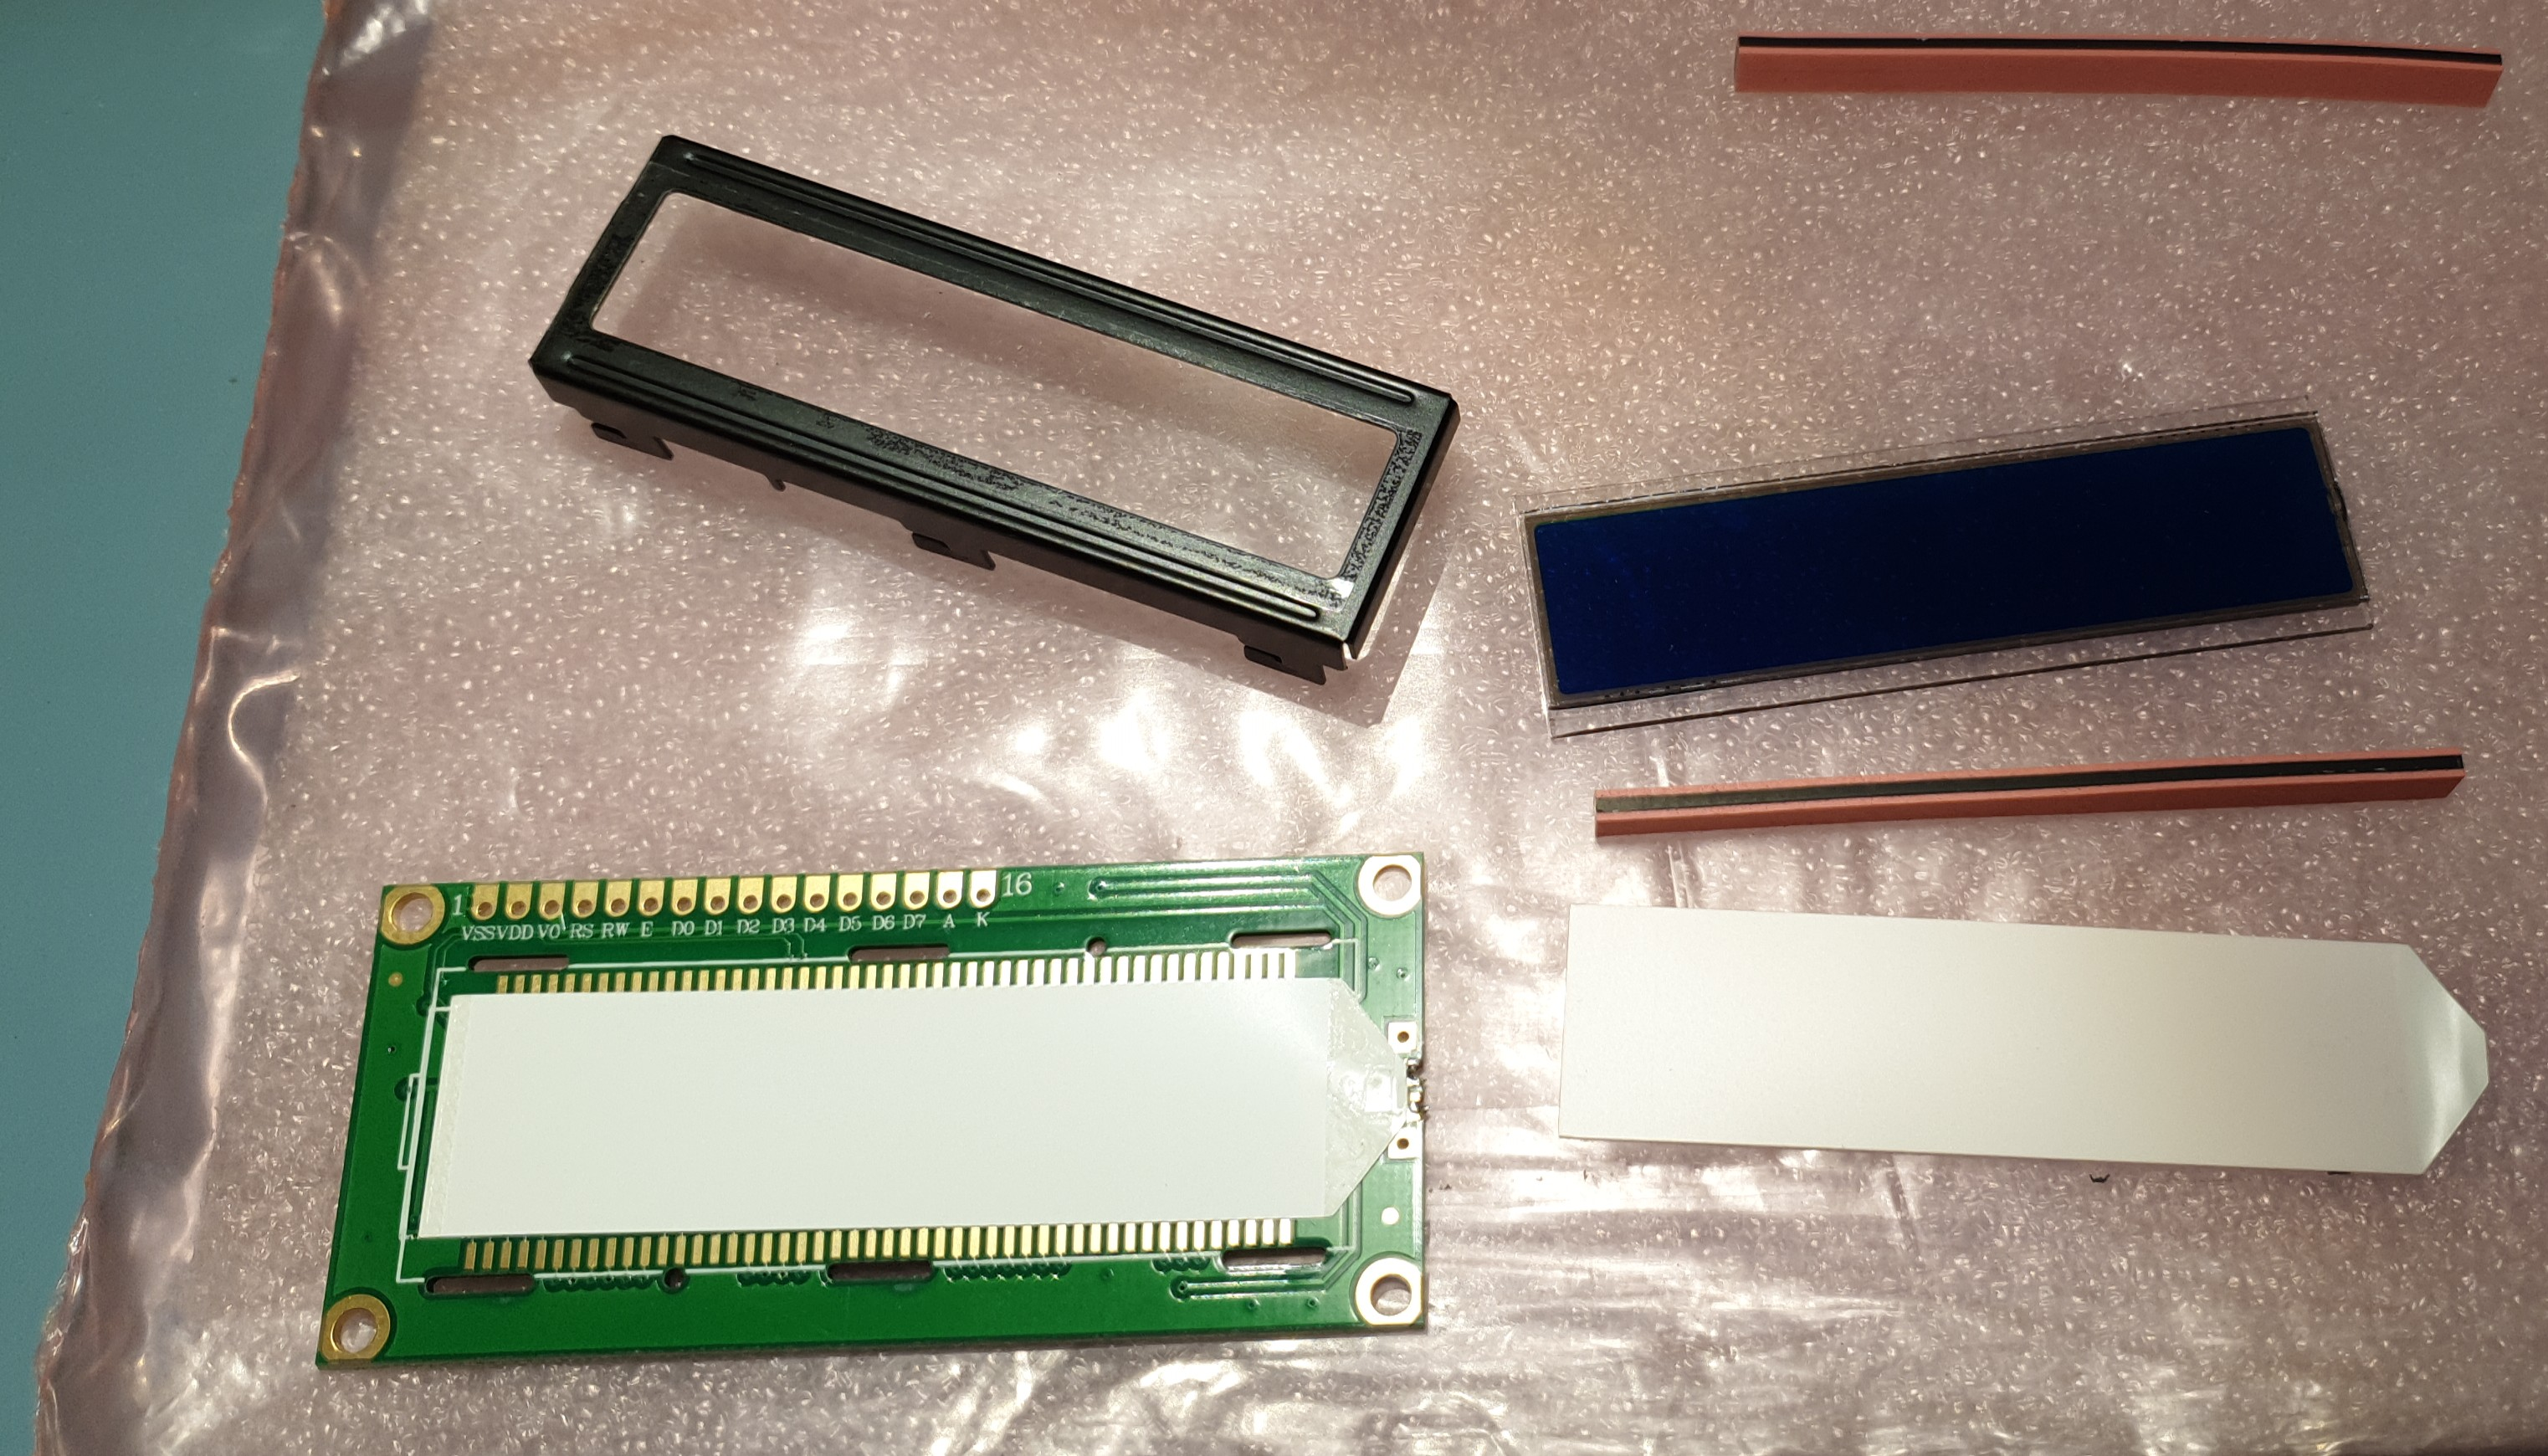
\includegraphics[width=\textwidth]{LCD-mod-pieces}};

        \begin{scope}[
            x={($1*(image.south east)$)},
            y={($1*(image.north west)$)}
        ]
            % grid
            %\draw[lightgray,step=0.1] (image.south west) grid (image.north east);

            \draw[stealth-, very thick,green] (0.5,0.2) -- ++(0.10,-0.10)
                node[right,black,fill=white]{\small spodní vrstva BLU};

            \draw[stealth-, very thick,green] (0.9,0.24) -- ++(-0.02,-0.07)
                node[left,black,fill=white]{\small horní vrstva BLU};

            \draw[very thick,green] (0.10,0.05) rectangle (0.58,0.45)
                node[below left,black,fill=white]{\small DPS};

            \draw[very thick,green] (0.59,0.48) rectangle (0.95,0.80)
                node[below left,black,fill=white]{\small open cell};

            \draw[very thick,green] (0.20,0.50) rectangle (0.58,0.92)
                node[below left,black,fill=white]{\small rámeček};

            \draw[latex-, very thick, green] (0.70,0.95) edge (0.60,0.97)
                (0.65,0.45) -- (0.60,0.97)
                node[left,black,fill=white]{\small Zebra strip (elastomerový konektor)};

            \node at (1,0) [above left, black,fill=white] {Na obrázku chybí plexisklo z BLU.};
        \end{scope}
    \end{tikzpicture}
    \caption{Výměna LED v podsvícení LCD}
    \label{fig:LCD modifikace}
\end{figure}

Úprava spočívá v rozebrání displeje, vyjmutí plexiskla z BLU a vylomení
přilepené bílé LED. Displej je poté složen a na jeho DPS je připájena červená
\num{3}\si{\milli\meter} LED, která je vložena do dutiny v plexiskle.


\subsection{Grafické konfigurační rozhraní budíku}
Na displeji jsou zobrazována textová data s jednoduchými grafickými ikonkami
(\num{5 x 8} obrazových bodů). Uživatel zařízení ovládá pomocí otočného
enkodéru s tlačítkem aktivovaným stisknutím jeho osy. Je-li podsvícení displeje
zhasnuté, dojde při prvním otočení enkodéru či stisku tlačítka k rozsvícení
v nočním režimu. Jas podsvitové LED je minimální a s rozhraním budíku ještě
není možné pracovat. Další stisk tlačítka či otočení ovládacího prvku vede
k rozsvícení na maximální jas a odblokování interakce.
Po \num{10} sekundách neaktivity uživatele je podsvícení displeje opět
zhasnuto.

Otáčením ovládacího prvku se po displeji pohybuje kurzor, jehož pozice je
indikována podtržením (rozsvícením nejnižšího řádku obrazových bodů) daného
znaku. Většina znaků proto využívá pouze vyšších \num{7} řádků. Ne všechny
znaky lze tímto způsobem vybrat, kurzor lze umístit pouze pod interaktivní
prvky. Existují 3 typy těchto prvků:
\begin{itemize}[nosep]
    \item tlačítka, která slouží k přechodu na jinou obrazovku,
    \item přepínače, které mají pouze dva stavy (zapnuto / vypnuto),
    \item výběrová menu, která mají více stavů (například číslo v rozsahu
        \numrange{0}{60}).
\end{itemize}

Při stisku tlačítka ovládacího prvku s kurzorem umístěným pod znakem s významem
tlačítka dochází k přechodu na jinou obrazovku (jiný pohled) a překreslení
displeje.

Stiskem ovládacího prvku při výběru přepínače dochází ke změně stavu tohoto
přepínače; tato změna je indikována změnou jeho znaku. Malá písmena značí
vypnutý přepínač, zatímco velká písmena jsou použita pro zapnuté přepínače.
Pokud je přepínač reprezentován číslicí, je ve vypnutém stavu nahrazen znakem
\textLCD{1}!-!.

Při stisku ovládacího prvku s kurzorem umístěným pod výběrovým menu dochází
k přechodu do režimu výběru. První ze znaků reprezentujících toto menu se
rozbliká (je střídavě nahrazován znakem \textLCD{1}!{fcur} !). Otáčením
ovládacího prvku se provádí výběr z prvků v tomto menu (nebo inkrementace /
dekrementace čísla). Volba je potvrzena stiskem ovládacího prvku, blikání znaku
ustává a otáčení volicího prvku opět pohybuje běžným kurzorem.

\begingroup
%\renewcommand{\arraystretch}{1.5}
\begin{longtable}{
        >{\centering\arraybackslash}m{50mm}
        m{\textwidth - 50mm - 4\tabcolsep - 3\arrayrulewidth}
    }
    \caption{Přehled obrazovek/pohledů grafického rozhraní budíku\label{tab:GUI screens}}
    \\
    \toprule
    Obrazovka
    & Vysvětlení
    \\
    \midrule
    \endfirsthead
    \caption[]{(pokračování)}\\
    \toprule
    Obrazovka
    & Vysvětlení
    \\
    \midrule
    \endhead
    \bottomrule
    \endfoot
    home
    \par\smallskip
    \LCD{2}{16}!04-03 7 00:05:30!
               !{bell}{timer} RTC i    00l !
        &
            Hlavní (domovská) obrazovka

            První řádek:
            \begin{itemize}[nosep]
                \item datum: [2022]-04-03,
                \item den v týdnu: 7. (neděle),
                \item čas: 00:05:30.
            \end{itemize}

            Druhý řádek:
            \begin{itemize}[nosep]
                \item tlačítka pro přechod na ostatní obrazovky:
                    \textLCD{1}!{bell} !~-- alarms,
                    \textLCD{1}!{timer} !~-- timer,
                    \textLCD{3}!RTC! -- RTC,
                \item přepínač režimu inhibit: \textLCD{1}!i! (vypnuto) / \textLCD{1}!I! (zapnuto),
                \item nastavení jasu stmívatelné LED (\numrange{0}{25}),
                \item ovládání světla lamp: \textLCD{1}!l! (vypnuto) / \textLCD{1}!L! (zapnuto).
            \end{itemize}
            \\
    alarms
    \par\smallskip
    \LCD{2}{16}!{home}0/5 12---67 OFF!
               !12:34+01*1  25lS!
        &
            Nastavení budicích časů

            První řádek:
            \begin{itemize}[nosep]
                \item \textLCD{1}!{home} !~-- přechod na obrazovku home,
                \item index času buzení: 0,
                \item index posledního času buzení: 5,
                \item dny v týdnu: \numlist{1;2;6;7},
                \item stav aktivace:
                    \textLCD{3}!OFF!~-- deaktivovaný,
                    \textLCD{3}!SGL!~-- aktivovaný pouze pro jedno buzení,
                    \textLCD{3}!RPT!~-- aktivovaný pro opakované buzení,
                    \textLCD{3}!SKP!~-- deaktivovaný pro jedno následující
                        buzení, poté přejde do \textLCD{3}!RPT!.
            \end{itemize}

            Druhý řádek:
            \begin{itemize}[nosep]
                \item čas buzení: 12:34,
                \item čas funkce \uv{dospat} (\SIrange{0}{99}{\minute}): \SI{1}{\minute},
                \item maximální počet použití funkce \uv{dospat} (\numrange{0}{9}): \num{1},
                \item jas stmívatelné LED (\numrange{0}{25}): \num{25},
                \item rozsvícení lampy: ne,
                \item akustické buzení: ano, přerušovaným pískáním.
                    Další hodnoty:
                    \textLCD{1}!s!~-- ne,
                    \textLCD{1}!0!--\textLCD{1}!9!~-- melodie \numrange{0}{9},
                    \textLCD{1}!A!--\textLCD{1}!F!~-- melodie \numrange{10}{15}.
            \end{itemize}
        \\
    timer
    \par\smallskip
    \LCD{2}{16}!     Timer      !
               !{home}{timer} 00:12:34 00lb!
        &
        Nastavení časovače

        Druhý řádek
        \begin{itemize}[nosep]
            \item \textLCD{1}!{home} !~-- přechod na obrazovku home,
            \item \textLCD{1}!{timer} !~-- tlačítko pro spuštění
                a zastavení časovače,
            \item čas časovače: 00:12:34,
                \item jas stmívatelné LED (\numrange{0}{25}): \num{0},
                \item rozsvícení lampy: ne,
                \item akustické buzení \textLCD{1}!b! (ne) / \textLCD{1}!B! (ano, přerušovaným pískáním): ne.
        \end{itemize}
        \\
    RTC
    \par\smallskip
    \LCD{2}{16}!{cancel}{apply}RTC 7 21:48:16!
               !2022-04-03      !
        &
        Nastavení hodin reálného času

        První řádek:
        \begin{itemize}[nosep]
            \item \textLCD{1}!{cancel} !~-- přechod na obrazovku home bez
                uložení změn,
            \item \textLCD{1}!{apply} !~-- přechod na obrazovku home po
                uložení změn,
            \item den v týdnu: 7 (neděle),
            \item čas: 21:48:16.
        \end{itemize}

        Druhý řádek:
        \begin{itemize}[nosep]
            \item datum: 2022-04-03.
        \end{itemize}
        \\
\end{longtable}
\endgroup
